\documentclass[a4paper, 12pt]{article}

\usepackage[T2A]{fontenc}
\usepackage[utf8]{inputenc}
\usepackage[english,russian]{babel}
\usepackage[left=15mm, top=20mm, right=15mm, bottom=20mm, nohead, nofoot]{geometry}

\usepackage{hyperref}
\usepackage{graphicx}
\usepackage{wrapfig}
\usepackage{afterpage}
\usepackage{amsmath, amsfonts, amssymb, amsthm, mathtools}
\author{Хомутов Андрей, группа Б06-903}
\title{ВПВ по курсу "Электричество и магнетизм" \\ Конденсатор на высоких частотах}
\date{22 декабря 2020 г.}
%%%%%%%%%%%%%%%%%%%%%%%%%%%%%%%%%%%%%%%%%%%%%%%%%%%%%%%%%%%%%%%%%%%%%%%%%
\usepackage{graphicx, wrapfig, subcaption, setspace, booktabs}
\usepackage[protrusion=true, expansion=true]{microtype}
\usepackage[english]{babel}
\usepackage{sectsty}
\usepackage{url, lipsum}
\newcommand{\HRule}[1]{\rule{\linewidth}{#1}}
\onehalfspacing
\setcounter{tocdepth}{5}
\setcounter{secnumdepth}{5}
%%%%%%%%%%%%%%%%%%%%%%%%%%%%%%%%%%%%%%%%%%%%%%%%%%%%%%%%%%%%%%%%%%%%%%%%%


\begin{document}

\title{ \normalsize \textsc{Лабораторная работа по физической химии}
		\\ [4.0cm]
		\HRule{0.5pt} \\ [0.3cm]
		\LARGE \textbf{{Изучение свойств электродов}}
		\HRule{0.5pt} \\ [0.1cm]
		\normalsize  \vspace*{18\baselineskip}}

\date{}

\author{Шамарина Екатерина, Б06-903 \\
		Хомутов Андрей, Б06-903 \\
ФБМФ, 2021\\ }

\maketitle
\thispagestyle{empty}
\newpage
%%%%%%%%%%%%%%%%%%%%%%%%%%%%%%%%%%%%%%%%%%%%%%%%%%%%%%%%%%%%%%%%%%%%%%%%%
\section*{Цели работы} 
\begin{enumerate}
    \item Знакомство  с  понятием  лимитирующей  стадии  электрохимической  реакции  и двумя принципиально разными причинами изменения потенциала электрода в условиях протекания тока –при быстрой и медленной электрохимической стадии
    \item Получение хлорсеребряного электрода и изучение его свойств
    \item Исследование свойств платинового электрода в условиях его поляризуемости и обратимости.  Оценка  ключевых  параметров  диффузионной  и  кинетической стадий электрохимических реакций.
\end{enumerate}
%%%%%%%%%%%%%%%%%%%%%%%%%%%%%%%%%%%%%%%%%%%%%%%%%%%%%%%%%%%%%%%%%%%%%%%%%
 
%\section{Теоретическая часть}
%\subsection{...}



\section{Практическая часть}
\subsection{Получение и проверка работы хлорсеребряных электродов}

В ячейке 0.1M HCl. Используется трёхэлектродная схема:

Рабочий электрод(+) : Ag/AgCl  

Противоэлектрод(-) : Pt  

Электрод сравнения(-) : Ag/AgCl (в 3.5M KCl) \newline
Серебряная проволока предварительно очищается от старого слоя AgCl с помощью катодной поляризации: например, в режиме линейной развертки потенциала от 0 до -1500 мВ со скоростью 10 мВ/с. Рез-ты на Рис.1

\begin{figure}[h!]
    \begin{center}
    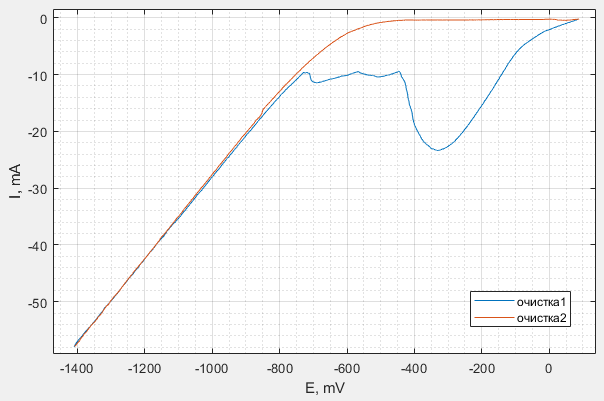
\includegraphics[width=0.7\textwidth]{1 очистка.png}
    \end{center}
    \caption{ВАХ очистки ХС электрода}
\end{figure}

Реакции на электродах: \newline
WE(К) : $AgCl + e^- \rightarrow Ag + Cl^-$ \newline
CE(А) : $2H_{2}O - 4e^- \rightarrow 4H^+ + O_2 \uparrow$

При втором проходе(электрод уже очищен, представляет собой серебряную проволочку) на участке нулевого тока электрод работает как поляризуемый. Далее(после -500мВ) ВАХ становится линейной из-за прохождения на электроде другой реакции: $H^+ + e^- \rightarrow \frac{1}{2} H_2 \uparrow$. Что можно наблюдать по выделению пузырьков на серебрянном электроде. (Линейность из-за того, что фарадеевское сопротивление мало => лимитирующая стадия - дифузионная, а эквив. схема - резистор.) При первом проходе участок "ямы" соответствует восстановлению серебра на катоде.

Для создания слоя AgCl использовалась анодная поляризация серебряной проволоки в потенциостатическом режиме около 200 мВ относительно хлорсеребряного электрода сравнения (в 3,5 M растворе KCl). Во время процесса серебряная проволока потемнела до бурого цвета. 

Реакции на электродах: \newline
WE(А) : $Ag + Cl^- - e^- \rightarrow AgCl$ \newline
CE(К) : $H_{2}O + e^- \rightarrow OH^- + \frac{1}{2} H_2 \uparrow$

\subsection{Поляризуемые и неполяризуемые электроды}

В ячейке 60 мл 1M КCl. Используется трёхэлектродная схема:

Рабочий электрод(+) : Ag/AgCl (получен в Части 1)

Противоэлектрод(-) : Pt (с большой площадью)

Электрод сравнения(-) : Ag/AgCl (в 3.5M KCl) \newline
C помощью потенциостата проведено измерение циклической ВАХ для двух рабочих электродов:
1) Ag/AgCl электрода (от –150 до 150 мВ относительно хлорсеребряного
электрода сравнения) в растворе 1 М KCl;
2) Pt электрода (в диапазоне потенциалов от –900 до 1150 мВ относительно
хлорсеребряного электрода сравнения) в растворе 1 М KCl. \newline
(Потенциостатический режим работы, циклическая развертку потенциала по времени, скорость развертки – около 100 мВ/с, скорость регистрации – 13 точек в секунду, 5 циклов.)\newline
Результаты на Рис.2-4

\begin{figure}[h!]
    \begin{center}
    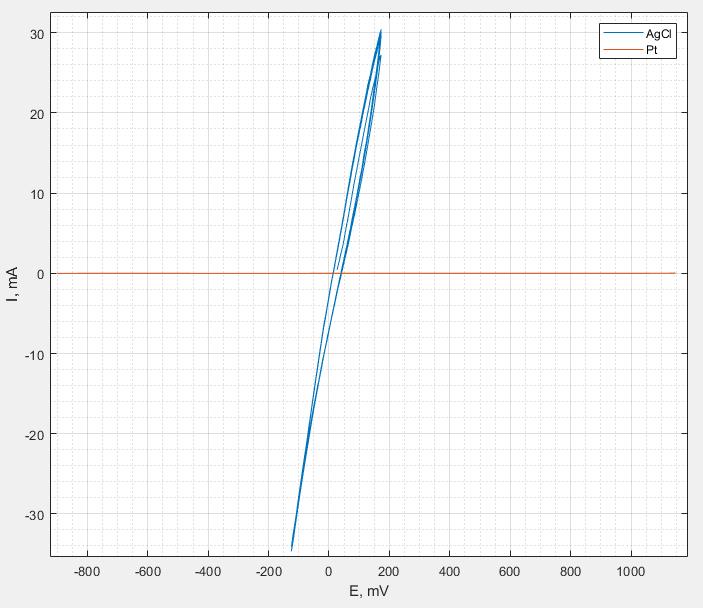
\includegraphics[width=0.8\textwidth]{2 both.png}
    \end{center}
    \caption{ЦВАХ обоих электродов}
\end{figure}

\subsubsection{Хлорсеребряный электрод}

Реакция на рабочем электроде: \newline
При катодном токе: $AgCl + e^- \rightarrow Ag + Cl^-$ \newline
При андоном токе: $Ag + Cl^- - e^- \rightarrow AgCl$ 

ЦВАХ соответствует неполяризуемому электроду.

\subsubsection{Платиновый электрод}

Реакция на рабочем электроде: \newline
При катодном токе: $H_{2}O+e^- \rightarrow OH^- +\frac{1}{2} H_2\uparrow$\newline
При андоном токе: $2H_{2}O - 4e^- \rightarrow 4H^+ + O_2 \uparrow$

ЦВАХ соответсвует поляризуемому электроду. (ИПЭ при потнециале -500..1000мВ отн.ХС.)

\begin{figure}[h!] %% ШАБЛОН ДЛЯ ДВУХ КАРТИНОК
\begin{center}
\begin{minipage}[h]{0.40\linewidth}
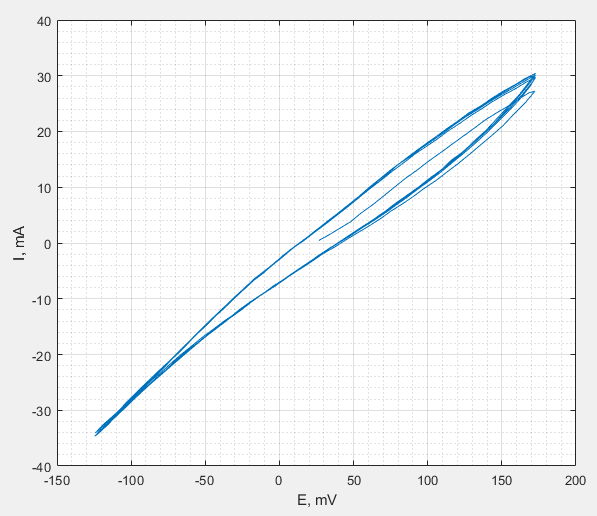
\includegraphics[width=1\linewidth]{2 AgCl.png}
\caption{ЦВАХ ХС электрода} %% подпись к рисунку
\label{ris:experimoriginal} %% метка рисунка для ссылки на него
\end{minipage}
\hfill 
\begin{minipage}[h]{0.40\linewidth}
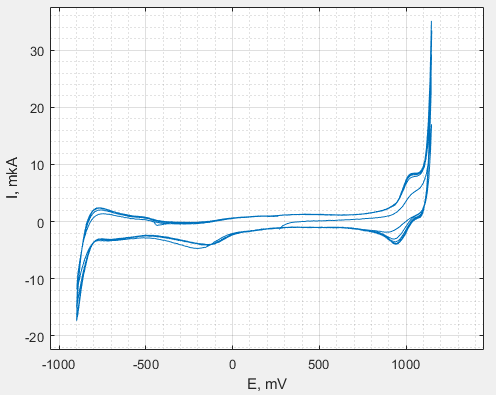
\includegraphics[width=1\linewidth]{2 Pt.png}
\caption{ЦВАХ платинового э-да}
\label{ris:experimcoded}
\end{minipage}
\end{center}
\end{figure}



\subsection{ОВР электрод}

В качестве рабочего электрода использовался платиновый электрод с малой площадью поверхности ($\sim \pi$ мм$^2$). В электрохимическую ячейку было добавлено 60мл 1M раствора KCl и по 1мл 0.1М растворов K$_3$[Fe(CN)$_6$] и K$_4$[Fe(CN)$_6$] (в дальнейшем K$_3$[Fe(CN)$_6$] и K$_4$[Fe(CN)$_6$]). Диапазон измерения катодной и анодной поляризационных кривых от -400 до 0 и от 0 до 400 мВ относительно ПРЦ соответственно при постоянной скорости перемешивания. Используемый режим - линейная развертка потенциала, скорость -  5мВ/с, диапазон тока - 200мкА.

Повторные измерения были проведены 5 раз при добавлении по 2мл K$_4$[Fe(CN)$_6$]. Кривые представлены на рис. 5. Также было рассмотрено влияние скорости перемешивания (см. рис. 6). Легко видеть что интенсивность колебаний при достижении предельного тока и сама величина этого тока прямо коррелируют со скоростью перемешивания. 

\begin{figure}[h!]
    \begin{center}
    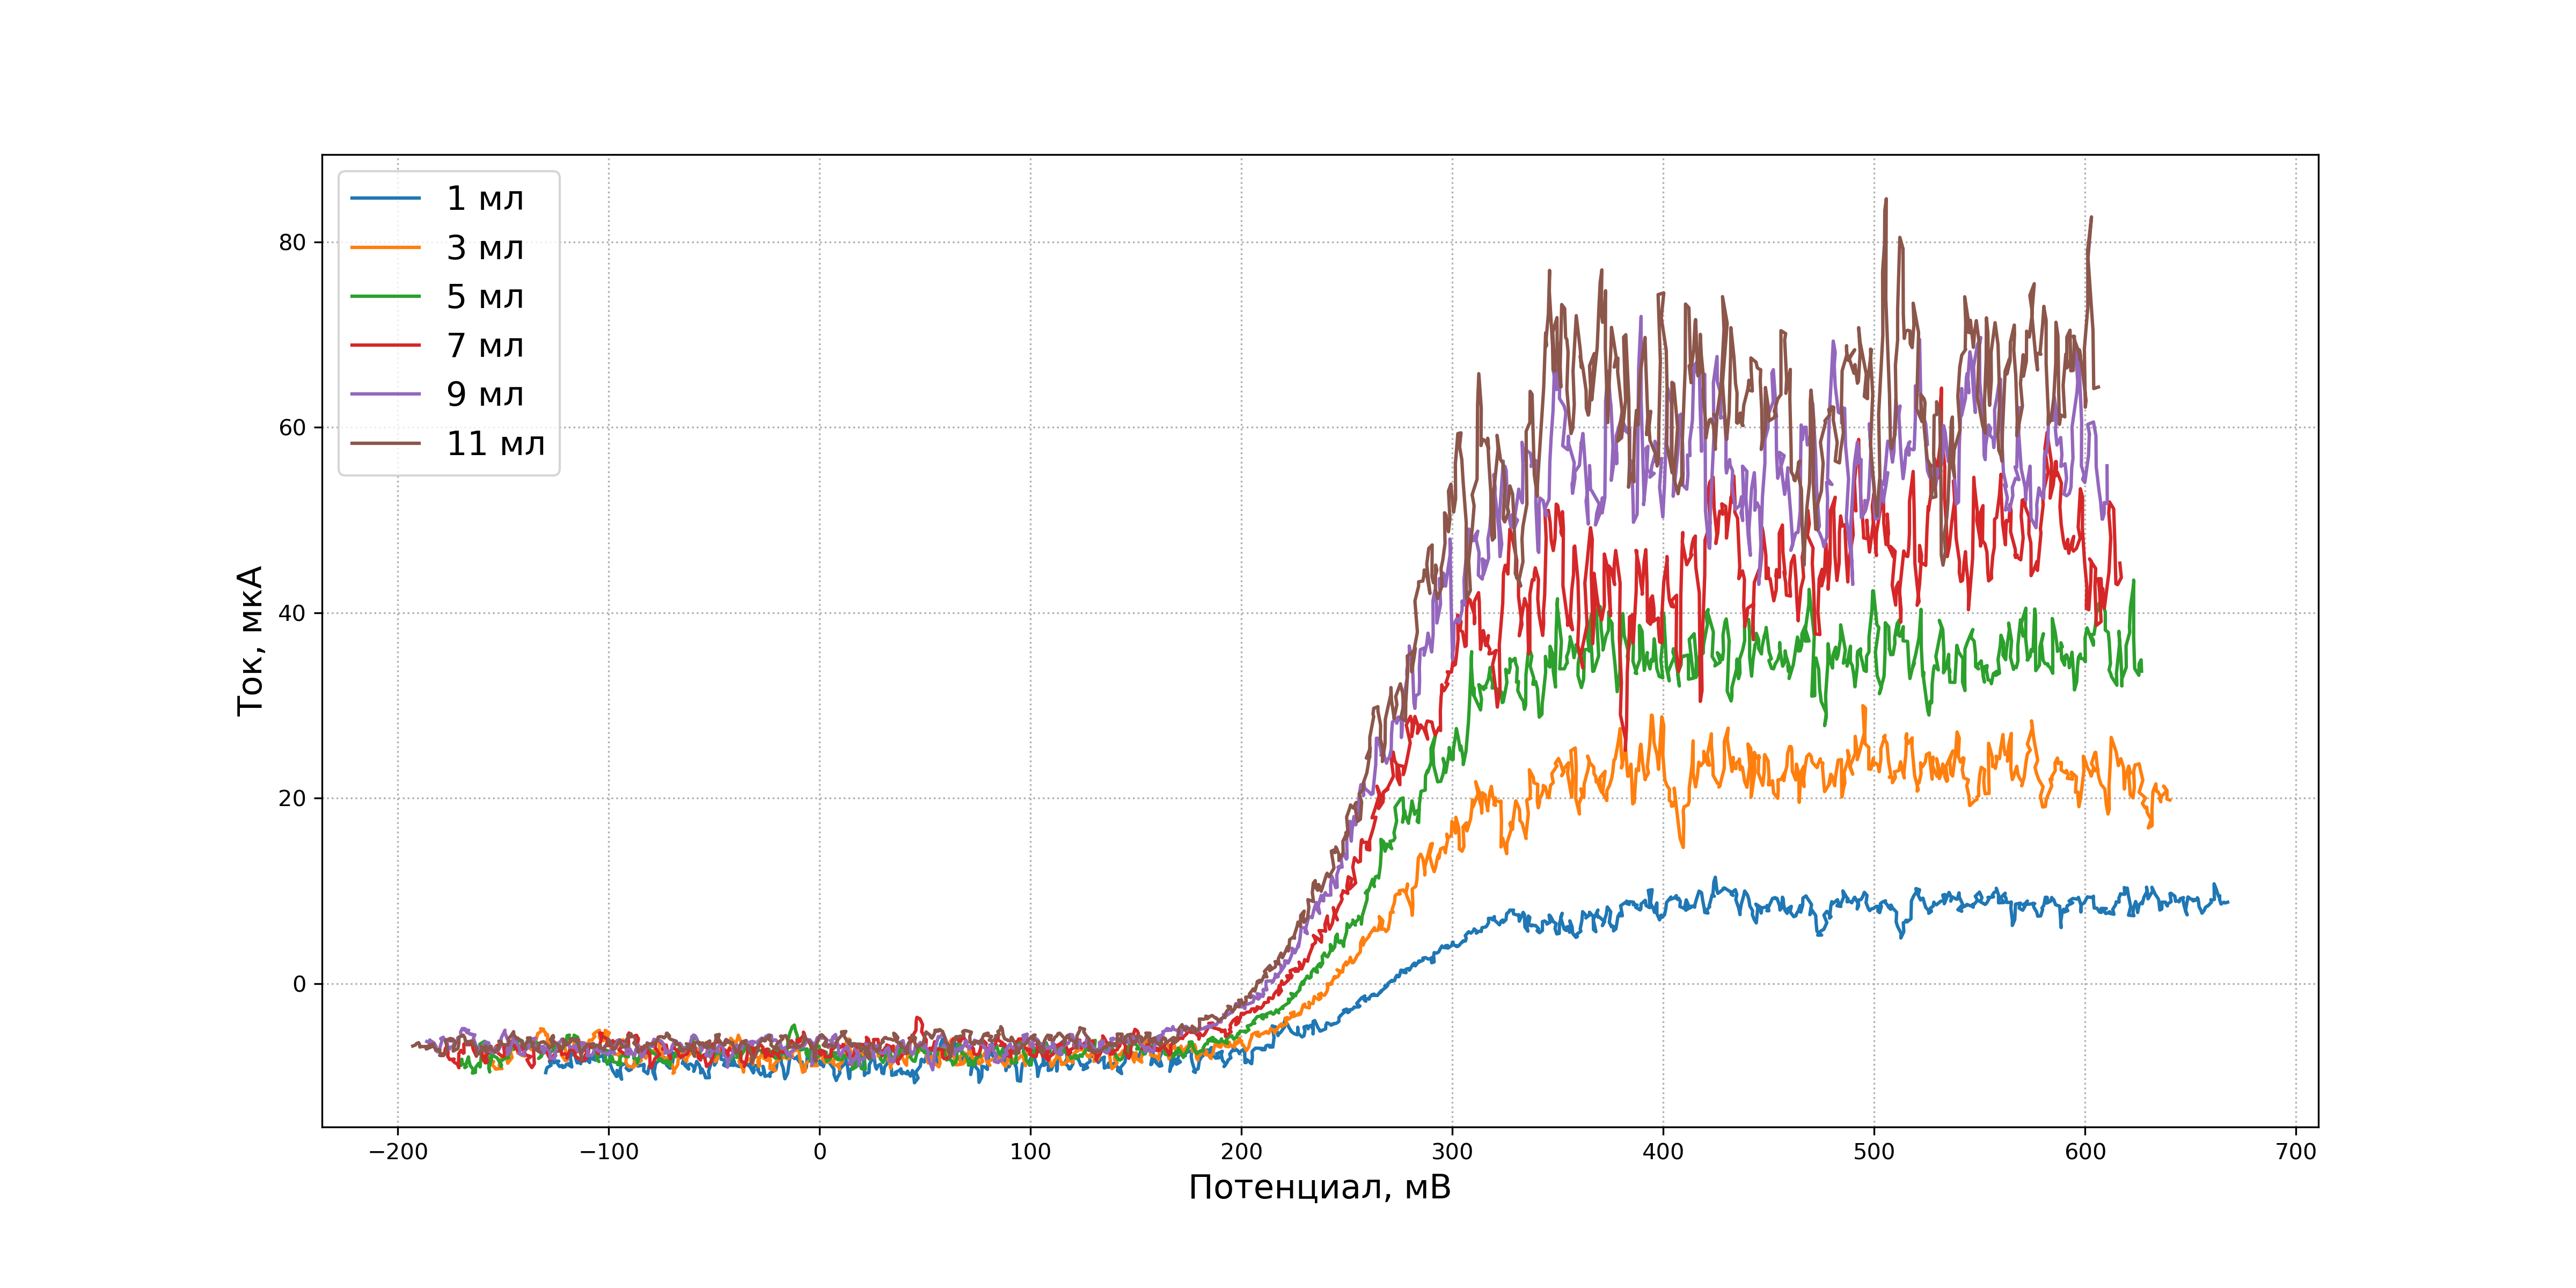
\includegraphics[width=1\textwidth]{curves.png}
    \end{center}
    \caption{Кривые поляризации для различных количеств добавленного K$_4$[Fe(CN)$_6$]}
\end{figure} % рисунок кривых

\begin{figure}[h!]
    \begin{center}
    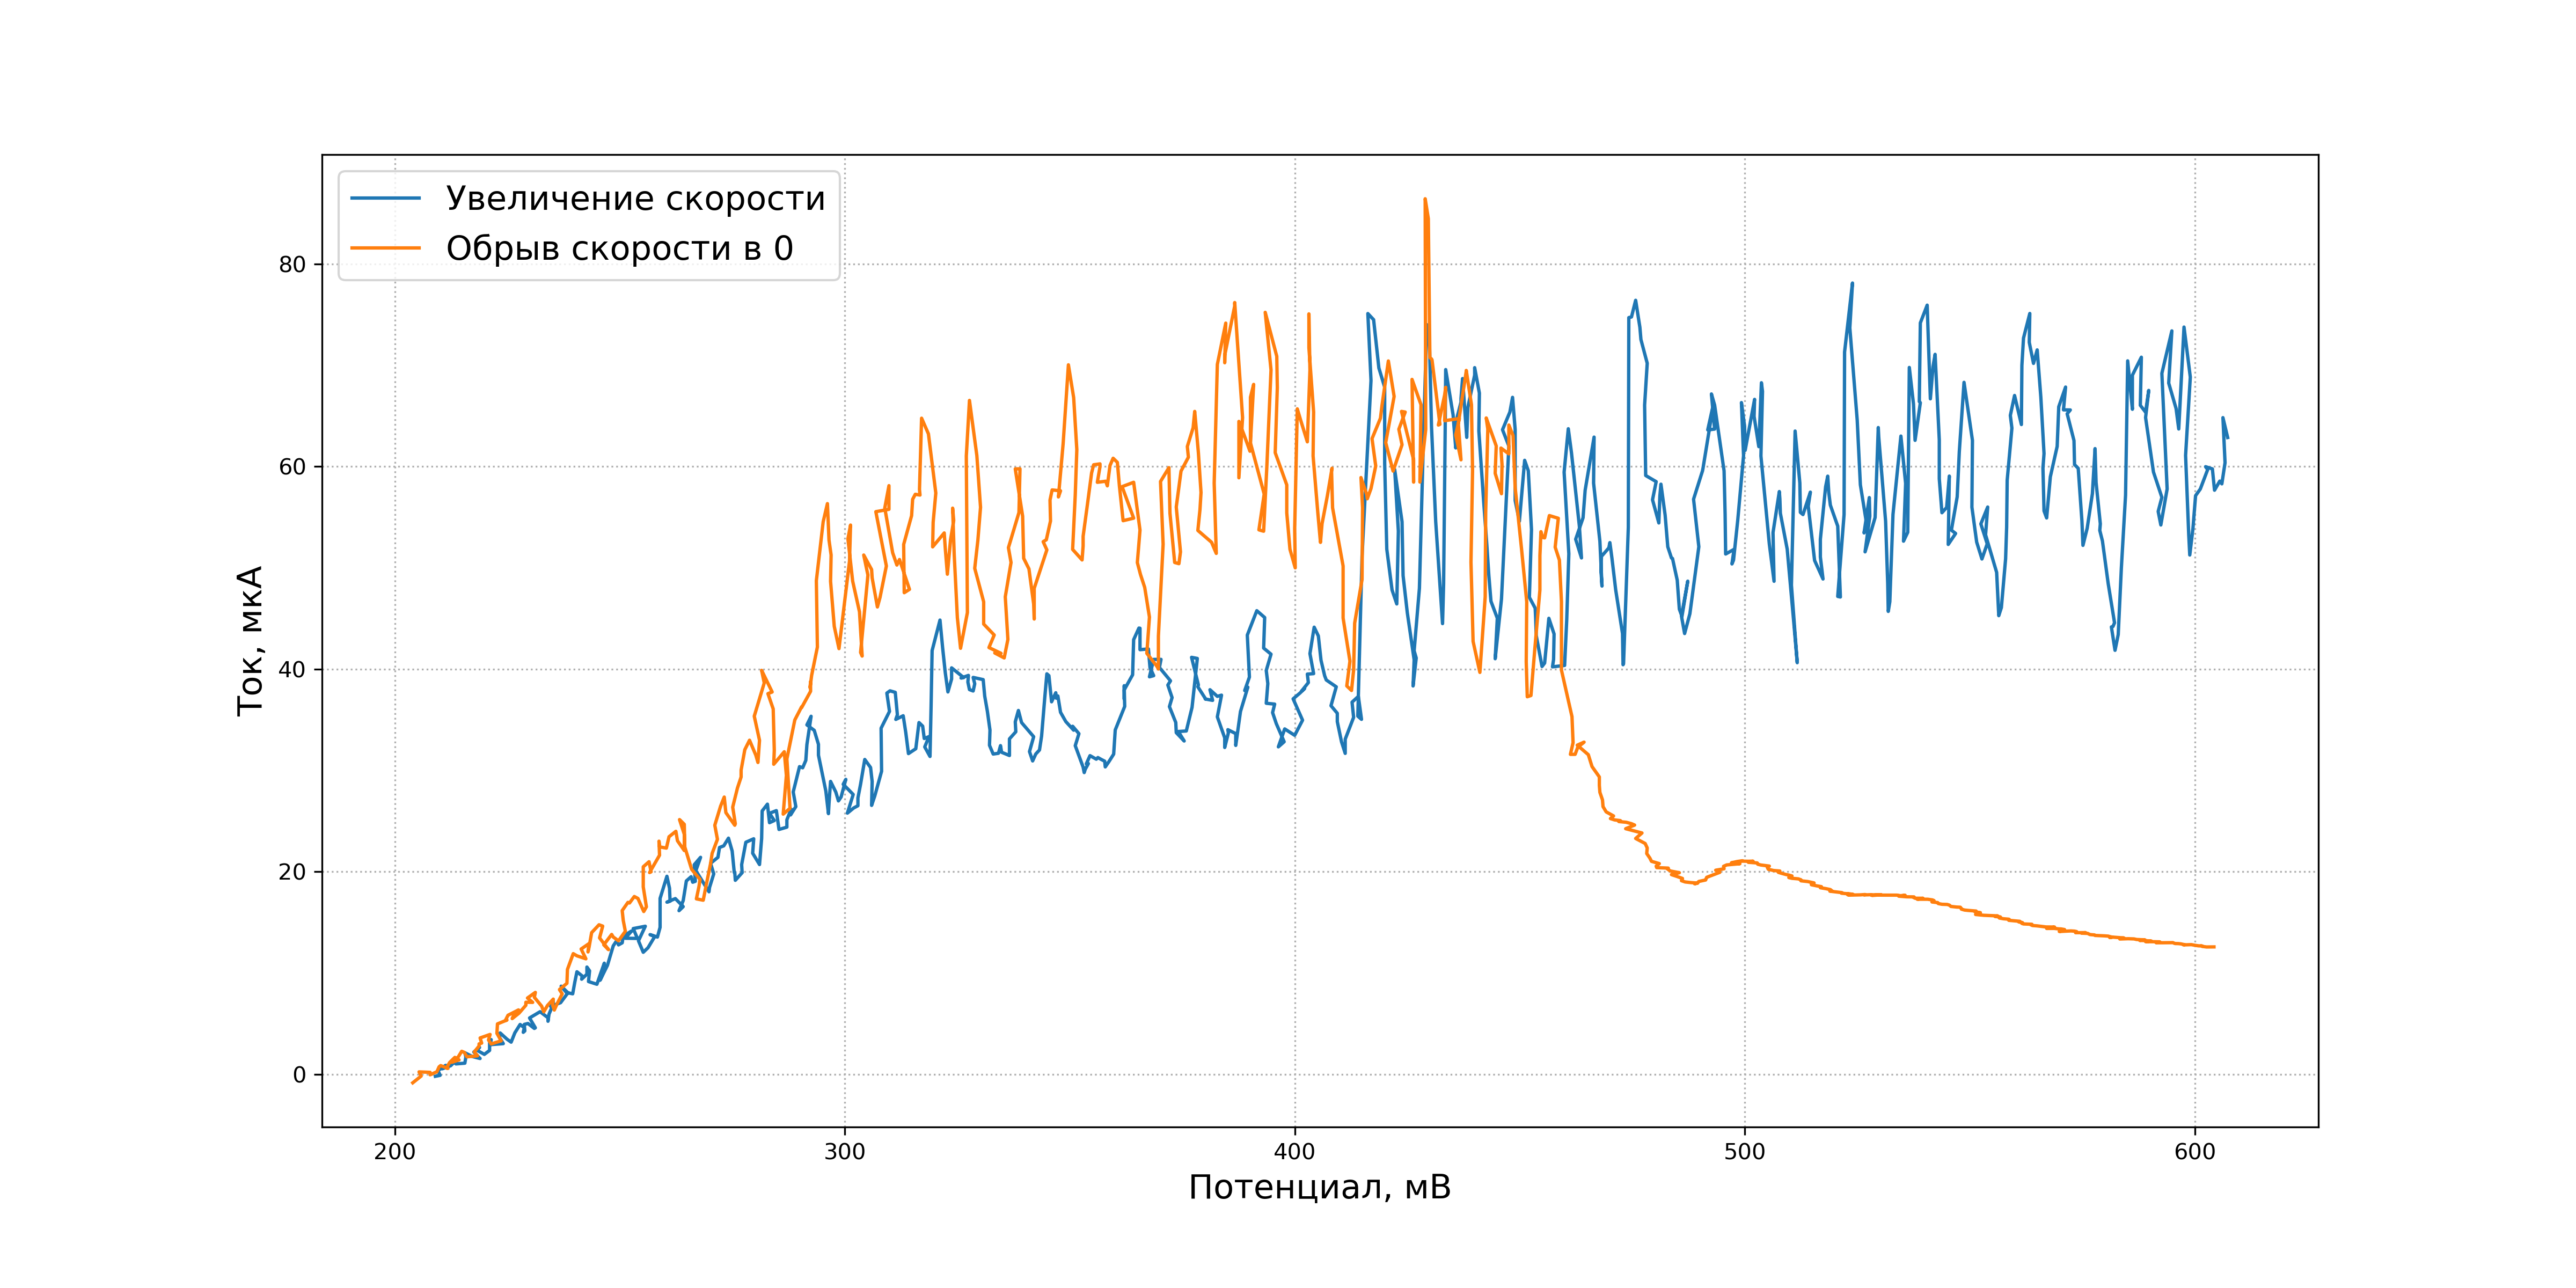
\includegraphics[width=1\textwidth]{обрыв.png}
    \end{center}
    \caption{Кривые поляризации при изменении скорости перемешивания для конечного раствора}
\end{figure} % рисунок для изменения скорости мешалки

Запишем процессы происходящие на рабочем электроде при его катодной и анодной поляризациях соответственно:

1. $\left[F e(C N)_{6}\right]^{3-}+e \rightarrow\left[F e(C N)_{6}\right]^{4-}$

2. $\left[F e(C N)_{6}\right]^{4-}-e \rightarrow\left[F e(C N)_{6}\right]^{3-}$

Построим график зависимости предельного диффузионного тока от концентрации K$_4$[Fe(CN)$_6$] и проведем ее линеаризацию (рис. 7, табл. 1). Отметим, что значение предельного катодного тока остается практически неизменным (~ -7 мкА), так как его величина определяется концентрацией K$_3$[Fe(CN)$_6$]. 

\begin{figure}[h!]
    \begin{center}
    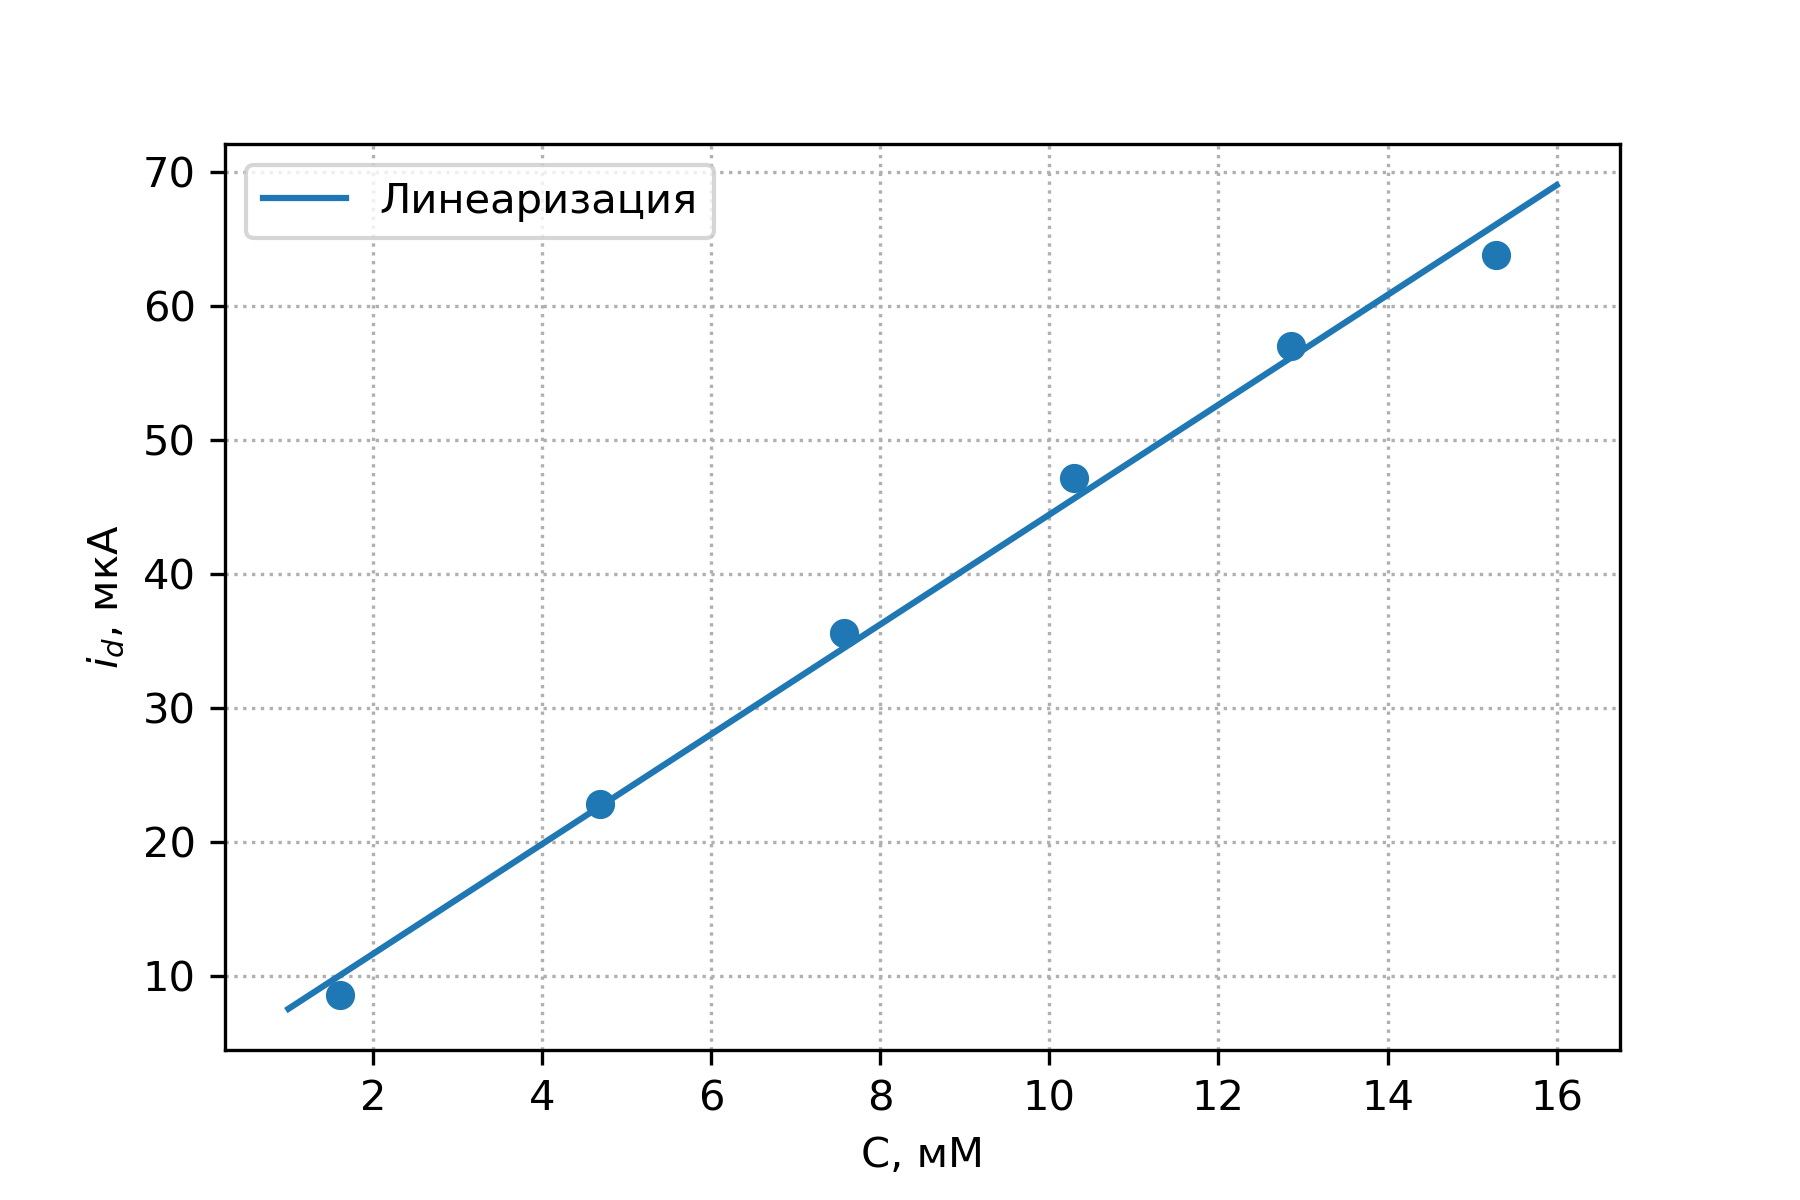
\includegraphics[width=0.8\textwidth]{I.png}
    \end{center}
    \caption{Зависимость предельного диффузионного тока от концентрации K$_4$[Fe(CN)$_6$]}
\end{figure}

Линейность этой зависимости следует из следующего выражения для предельного диффузионного тока:
$$i_{d}=-n F D \frac{c_{R}^{b}}{\delta},$$

где $c_{R}^{b}$ - концентрация восстановленной формы (для анодного тока) в объеме.

Таким образом, зная коэффициент наклона зависимости $i_{d}(c_{R}^{b})$, можно определить толщину диффузионного слоя\footnote{D(K4) =  0.739 $\cdot 10^{-5}$ см$^2$/с. Ньюмен Дж. Электрохимические системы, с. 260.}:
$$
\delta=\frac{F D  S}{k}= 54,7 \text{мкм}.
$$

Из уравения Нернста:
$$
E_{\mathrm{p}}=E^{0}-\frac{R T}{n F} \ln \left(\frac{C\left(K_{4}\left[F e(C N)_{6}\right]\right)}{C\left(K_{3}\left[F e(C N)_{6}\right]\right)}\right)
$$

Таким образом, построив зависимость стационарного потенциала от логарифма отношения концентраций K$_4$[Fe(CN)$_6$] и K$_3$[Fe(CN)$_6$], можно по углу наклона определить n:
$$
n=\frac{R T}{k F}=0.93 \simeq 1
$$

\begin{figure}[h!]
    \begin{center}
    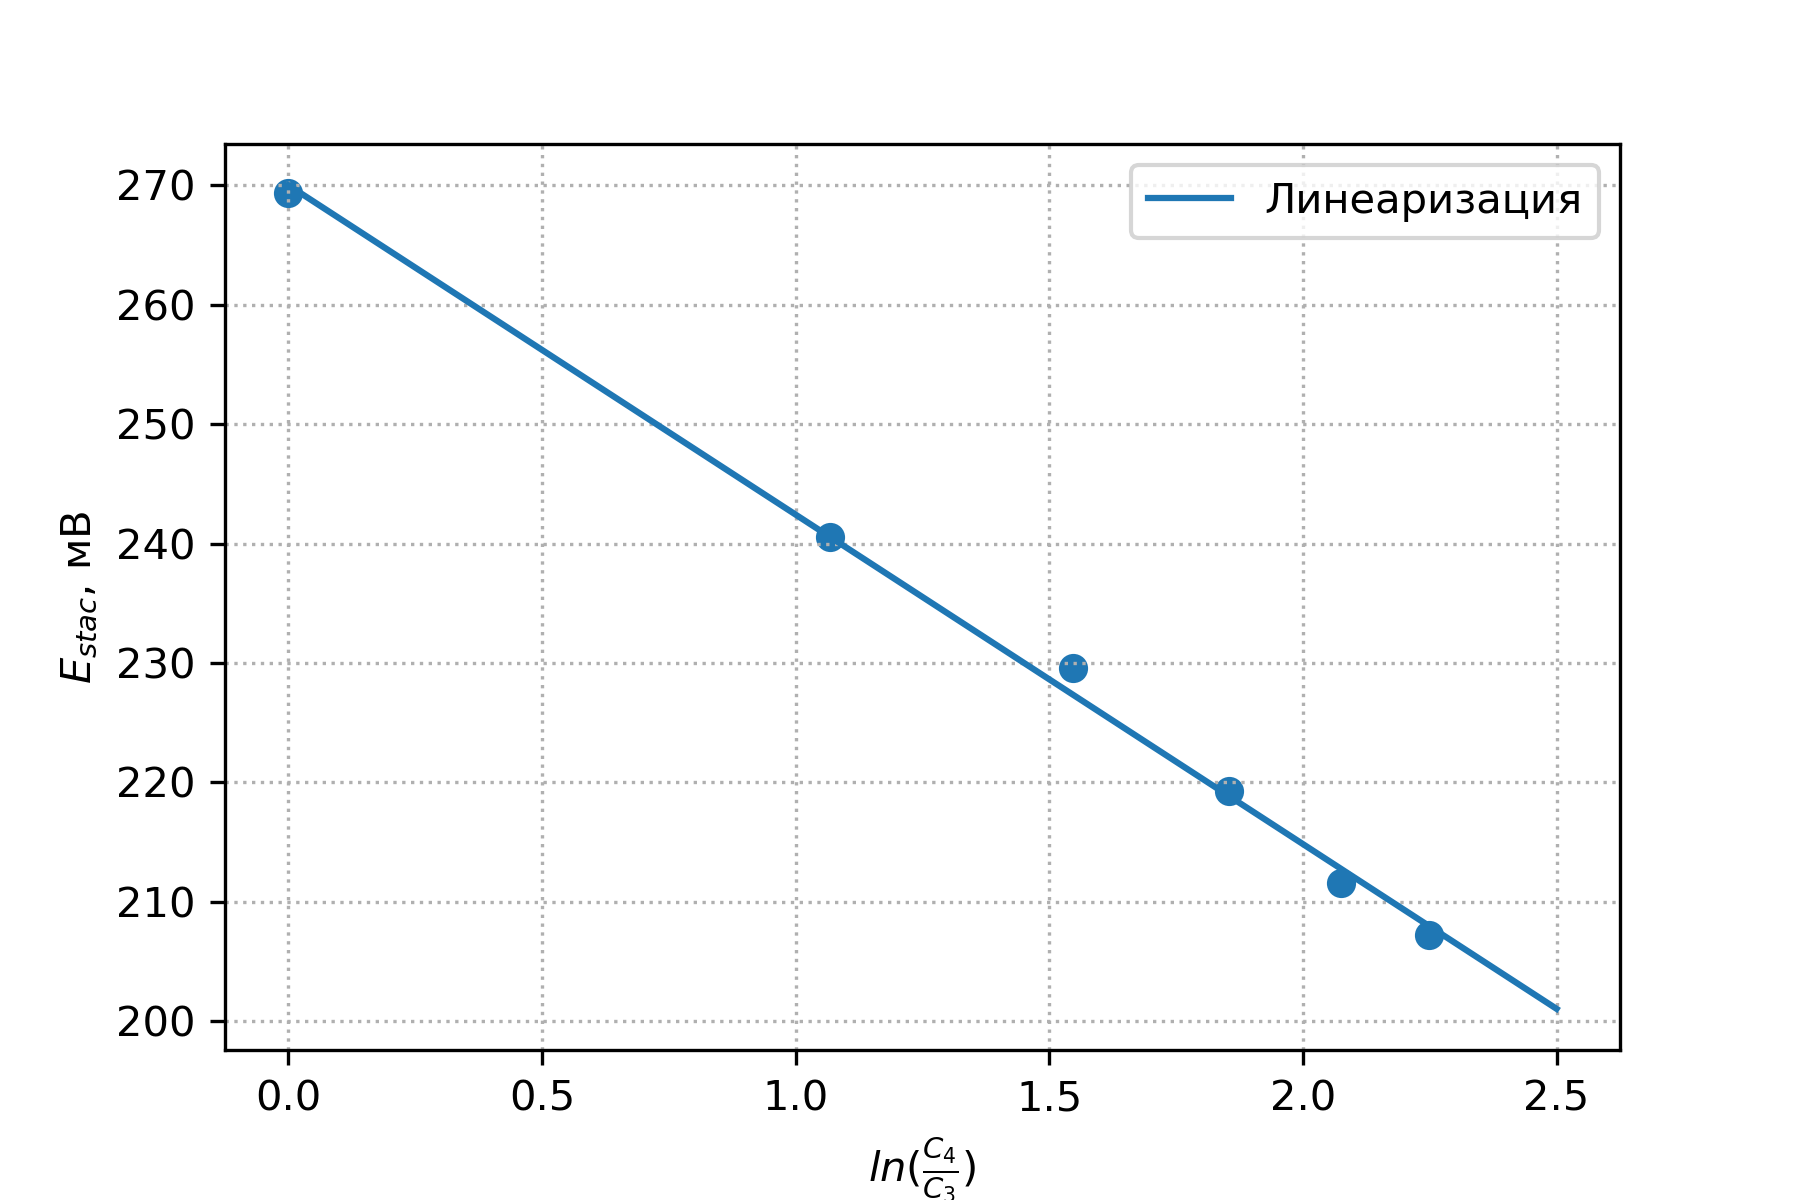
\includegraphics[width=0.8\textwidth]{U.png}
    \end{center}
    \caption{Зависимость $E_{p}$(ln(С(K$_4$[Fe(CN)$_6$])/С(K$_3$[Fe(CN)$_6$])))}
\end{figure}

Оценим, максимальное количество K$_3$[Fe(CN)$_6$] образовавшегося из K$_4$[Fe(CN)$_6$] при регистрации поляризационной кривой. 
$$
\nu_{max} = \frac{I_d^{(11)} t}{F} = \frac{63.8 \cdot 10^{-6} \cdot 80}{96385} \simeq 53 \text{  нмоль}
$$

\begin{table}[h!]
\begin{center}
\caption{Предельные диффузионныые токи и равновесные потенциалы в зависимости от концентрации реагентов}
\begin{tabular}{|c|c|c|c|}
\hline
С(K$_4$[Fe(CN)$_6$]), мМ & С(K$_3$[Fe(CN)$_6$]), мМ & id,  мкА & Ep, мВ \\ \hline
1,61      & 1,61      & 8,6      & 269,34 \\ \hline
4,69      & 1,56      & 22,8     & 240,57 \\ \hline
7,58      & 1,52      & 35,6     & 229,57 \\ \hline
10,29     & 1,47      & 47,1     & 219,28 \\ \hline
12,86     & 1,43      & 57,0     & 211,6  \\ \hline
15,28     & 1,39      & 63,8     & 207,2  \\ \hline
\end{tabular}
\end{center}
\end{table}


\subsection{Диффузионный потенциал}
В режиме вольтметра была снята зависимость разности потенциалов между двумя хлорсеребряными электродами, помеещенными в 1М и 0.1М растворы HCl, соединенные фильтровальной бумажкой, смоченной 1М раствором HCl. Установившееся значение $\Delta E$ через час наблюдения составило 103.5 мВ.

Расчитаем теоретическое значение разности потенциалов. С учетом того, что после разбавления растворов в 100 раз (200 мкл, доведенные до 20 мл дистиллированной водой) электропроводности при 25 С получились равными 836 мкСм/см и 7190 мкСм/см, можно сделать вывод что отношение концентраций $\alpha = 8.6$. 
$$
\Delta E = \Delta E_{Nernst} + \Delta \varphi_{diff} = \frac{R T}{n F} \cdot \ln \frac{c_{2}}{c_{1}} \cdot(1 + \frac{D_{+}-D_{-}}{D_{+}+D_{-}}) = 90.6 \text{ мВ}.
$$



%%%%%%%%%%%%%%%%%%%%%%%%%%%%%%%%%%%%%%%%%%%%%%%%%%%%%%%%%%%%%%%%%%%%%%%%%
 \section{Выводы}
\begin{enumerate}
    \item Получен хлорсеребряный электрод, и изучены его свойства.
    \item С помощью потенциостата измерены ЦВАХ хлорсеребряного и платинового электродов. На их основании сделаны выводы о характере электродов: ХС - неполяризуемый, Pt - поляризуемый. 
    \item Для платинового ОВР электрода были сняты поляризационные кривые для различных концентраций восстановленной формы.
    \item По предельным значениям диффузионного тока была оценена толщина диффузионного слоя
    \item По стационарным значниям потенциала было подтверждено что количесто электронов, передаваемое в электрохимической реакции, равно 1.
    \item Было установлено что скорость перемешивания влияет как на величину колебаний тока около его предельного значения, так и на саму величину этого тока.
    \item Была измерена равновесная разность потенциалов между двумя хлорсеребряными электродами в растворах HCl различной концентрации, и расчитана теоретически через выражение для диффузионного потенциала.
\end{enumerate}

\end{document}


\section{Приложение}

\begin{figure}[h!]
    \begin{center}
    \includegraphics[width=0.8\textwidth]{xxx.png}
    \end{center}
    \caption{...}
\end{figure}

\begin{figure}[h!] %% ШАБЛОН ДЛЯ ДВУХ КАРТИНОК
\begin{center}
\begin{minipage}[h]{0.40\linewidth}
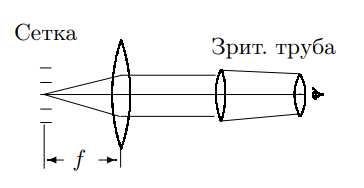
\includegraphics[width=1\linewidth]{plus_lens.PNG}
\caption{...} %% подпись к рисунку
\label{ris:experimoriginal} %% метка рисунка для ссылки на него
\end{minipage}
\hfill 
\begin{minipage}[h]{0.40\linewidth}
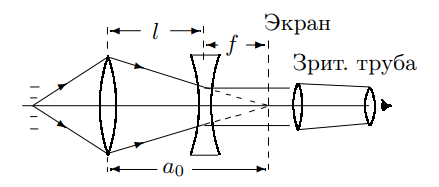
\includegraphics[width=1\linewidth]{minus_lens.PNG}
\caption{..}
\label{ris:experimcoded}
\end{minipage}
\end{center}
\end{figure}







\begin{table}[h!]
\begin{center}
\caption{...}
\begin{tabular}{|c|c|c|c|c|}

\end{tabular}
\end{center}
\end{table}






































